\chapter{Lab 2 Results: Attention Is Not All You Need}\label{app:lab2}

This appendix presents the experimental results from Lab~2, which tests whether each structural ingredient of a Transformer block is load-bearing. The method is systematic ablation: start with a working baseline, remove one ingredient, measure the damage.

\textbf{Task:} English morphological inflection (UniMorph). Four tags: PAST, GERUND, 3SG, PLURAL. $\sim$19k balanced pairs per tag. Vaswani-style encoder-decoder, 2+2 layers, $d_\text{model}=128$, 4 heads, FFN=512, pre-norm.

%----------------------------------------------------------------------
\section{Experiment 0: Vanilla Baseline}

\textbf{Question:} What is the ceiling performance before any ablation?

\textbf{Results:}

\begin{center}
\begin{tabular}{lcccc}
\toprule
 & \textbf{Pure Regular} & \textbf{Phonological} & \textbf{Irregular} & \textbf{Overall} \\
\midrule
Vanilla & 98.5\% & 98.1\% & 42.0\% & 97.1\% \\
\bottomrule
\end{tabular}
\end{center}

\begin{figure}[h]
\centering
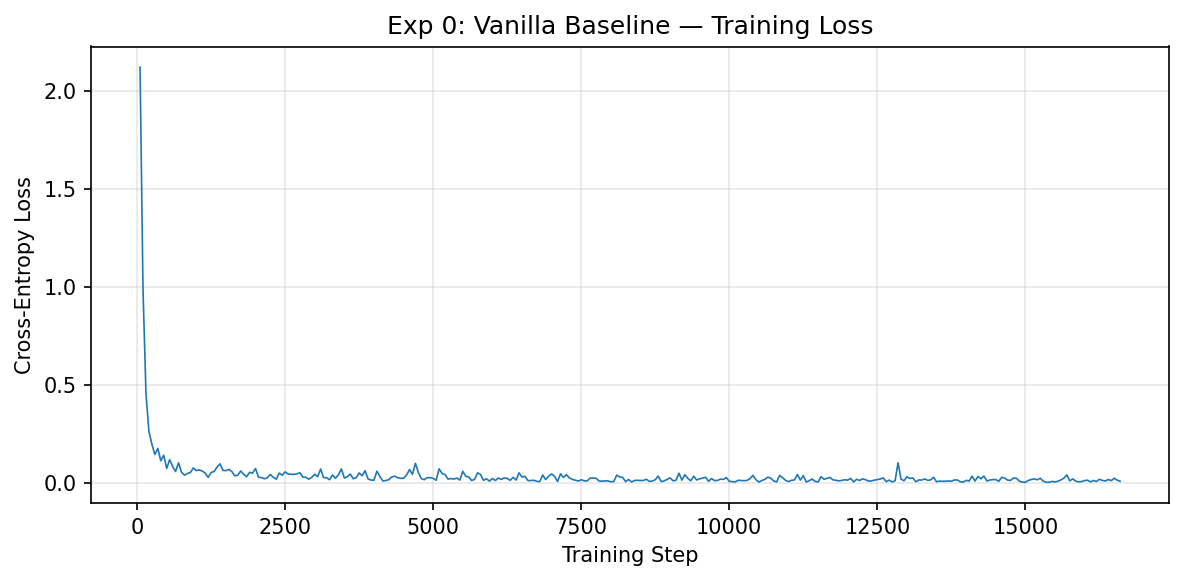
\includegraphics[width=0.6\textwidth]{labs/ch02/answers/exp0_baseline/train_curve.png}
\caption{Vanilla model training curve. Converges smoothly within 12 epochs.}
\label{fig:app-lab2-baseline}
\end{figure}

\textbf{Diagnosis:} The model handles rule-based inflection (regular, phonological) near-perfectly. Irregular forms require per-lemma lookup (\texttt{go}$\to$\texttt{went}), which is much harder---42\% sets the ceiling for this ablation series.

\textbf{Core insight:} The three-tier difficulty structure (regular $>$ phonological $>$ irregular) is pedagogically critical. It creates a \emph{sensitivity gradient} for ablation: regular forms are so easy that even crippled models can partially learn them, while irregular forms require the full expressive power of the architecture. This is why we report accuracy by category rather than a single overall number---the overall 97.1\% hides that irregulars are only 42\%. When we ablate components later, damage shows up first in irregular accuracy, then phonological, and finally regular. This makes the ablation results \emph{interpretable}: you can tell which capability was lost by looking at which tier degrades.

%----------------------------------------------------------------------
\section{Experiment 1: The Causal Mask Bug (Silent Failure)}

\textbf{Question:} What happens when the decoder causal mask is removed?

\textbf{Results:}

\begin{center}
\begin{tabular}{lcc}
\toprule
 & \textbf{Train Loss} & \textbf{Val Accuracy} \\
\midrule
With mask (correct) & 0.0169 & 97.1\% \\
Without mask (broken) & 0.0030 & 0.0\% \\
\bottomrule
\end{tabular}
\end{center}

\begin{figure}[h]
\centering
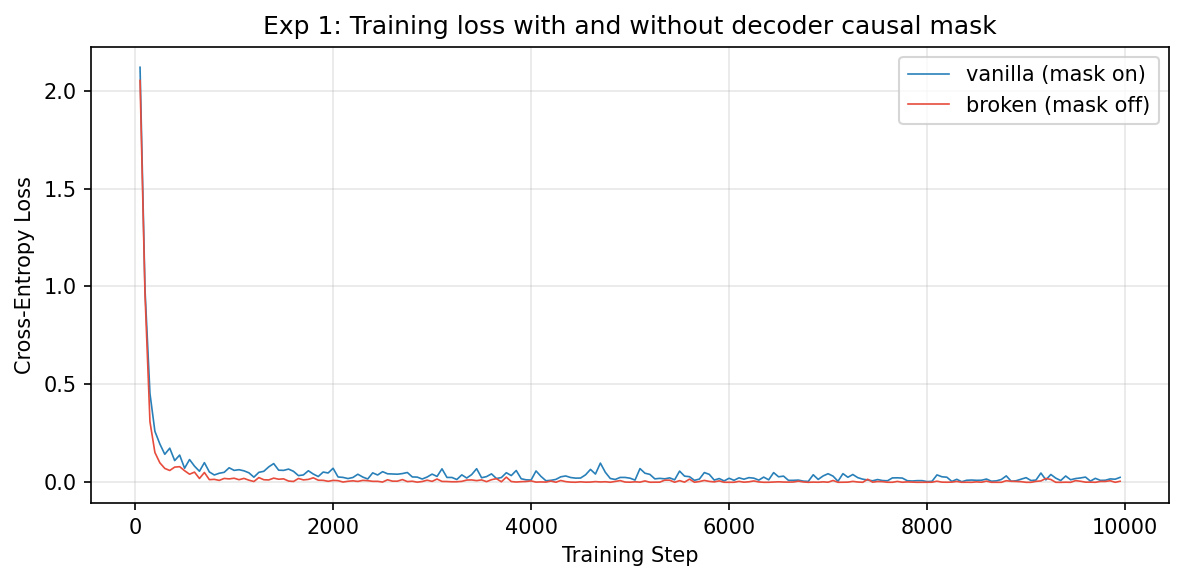
\includegraphics[width=0.65\textwidth]{labs/ch02/answers/exp1_mask/train_curves.png}
\caption{Training loss: the broken model (no causal mask) converges to \emph{lower} loss---but produces 0\% accuracy at inference.}
\label{fig:app-lab2-mask}
\end{figure}

\textbf{Diagnosis:} Without a causal mask, the decoder sees the ground-truth future during teacher forcing. It learns to copy the target one position ahead---trivial, hence lower loss. At inference, the future does not exist, and the model outputs degenerate strings (\texttt{wwwww}, empty outputs). \textbf{A low training loss is not evidence that a model has learned anything generalizable.}

\textbf{Core insight:} This is arguably the most important lesson in the entire lab series. The mask bug creates a \emph{train/test distribution shift that is invisible in the loss curve}. The model genuinely converges---loss drops smoothly, gradients are healthy, no NaN. Every metric says ``training succeeded.'' But the model learned a shortcut (copy from future) that only exists during teacher forcing. This pattern generalizes far beyond masks: any train-time information leak that vanishes at inference produces the same symptom. Examples in real research include: label leakage in train/test splits, future feature leakage in time-series, and auxiliary losses that provide shortcuts unavailable at deployment. The diagnostic discipline is always the same: \emph{when loss is suspiciously good, test generation quality before celebrating.}

%----------------------------------------------------------------------
\section{Experiment 2: Rank Collapse (Centerpiece)}

\textbf{Question:} Which ingredient prevents token representations from collapsing to a single vector?

\textbf{Setup:} Two parts. (A) Stack 24 layers of each ablation and measure mean cosine similarity at random init (no training). (B) Train each ablation on the inflection task.

\subsection{Part A: Rank Collapse at Initialization}

\begin{center}
\begin{tabular}{lc}
\toprule
\textbf{Configuration} & \textbf{Final-Layer Mean Cosine} \\
\midrule
Pure SAN (no residual, no FFN) & 1.000 \\
+ FFN only (no residual) & 1.000 \\
+ Residual only (no FFN) & 0.483 \\
Vanilla (residual + FFN) & 0.480 \\
\bottomrule
\end{tabular}
\end{center}

\begin{figure}[h]
\centering
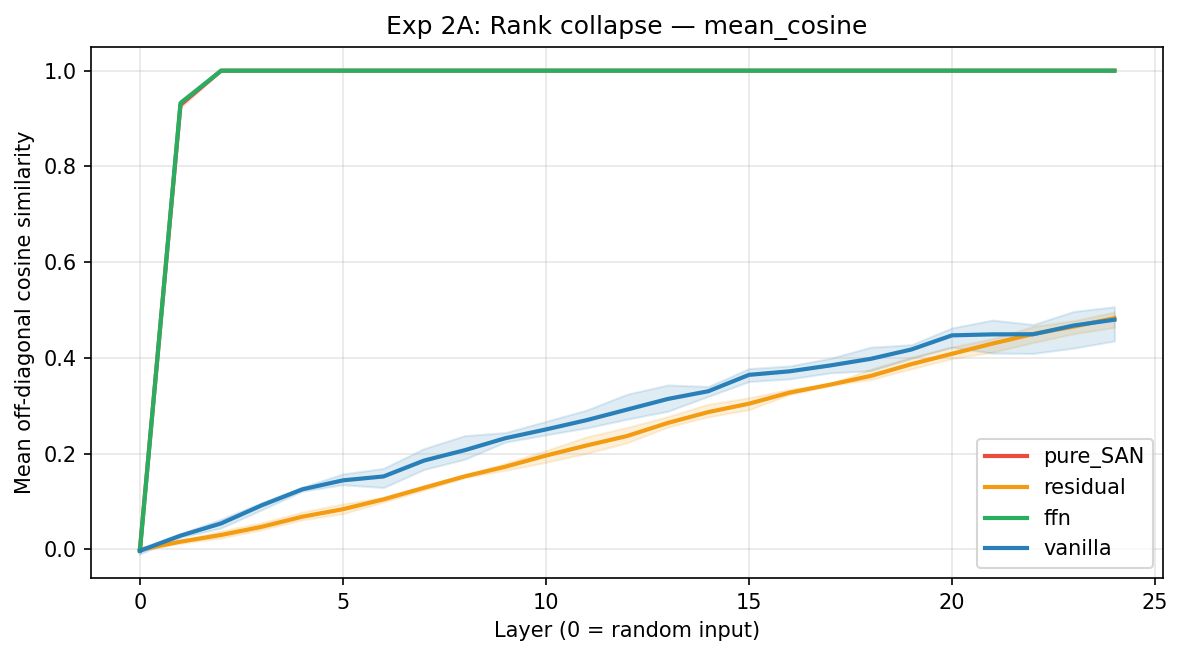
\includegraphics[width=0.7\textwidth]{labs/ch02/answers/exp2_rank_collapse/diagnostic_cosine.png}
\caption{Mean cosine similarity vs.\ depth. Pure SAN and FFN-only collapse to cosine=1.0 by layer 2 (rank-1 collapse). Residual connection prevents this.}
\label{fig:app-lab2-cosine}
\end{figure}

\textbf{Key finding:} FFN's per-token nonlinearity does NOT prevent collapse on its own. Only the residual connection preserves token diversity across depth.

\textbf{Why this is surprising:} The naive intuition says ``FFN adds nonlinearity, nonlinearity adds expressiveness, so FFN should prevent collapse.'' But the data shows the opposite: FFN-only still collapses to cosine=1.0. The reason is that self-attention without residual acts as an \emph{averaging} operator. Each token's representation becomes a weighted average of all visible tokens. After repeated averaging, all representations converge to the same point (rank-1). FFN applies a nonlinear transform \emph{to each token independently}---but if all tokens already look the same (post-collapse), applying the same function to identical inputs produces identical outputs. The FFN cannot ``un-collapse'' what attention already destroyed. Only the residual connection prevents collapse by ensuring each token retains its original identity alongside the attention-modified signal.

\subsection{Part B: Trained Accuracy}

\begin{center}
\begin{tabular}{lcccc}
\toprule
\textbf{Config} & \textbf{Pure Regular} & \textbf{Phonological} & \textbf{Irregular} & \textbf{Overall} \\
\midrule
Pure SAN & 75.5\% & 61.9\% & 1.1\% & 69.4\% \\
+ Residual only & 99.0\% & 96.9\% & 29.4\% & 96.7\% \\
+ FFN only & 0.0\% & 0.0\% & 0.0\% & 0.0\% \\
Vanilla & 98.5\% & 98.1\% & 42.0\% & 97.1\% \\
\bottomrule
\end{tabular}
\end{center}

\textbf{Diagnosis:}
\begin{itemize}
\item \textbf{Pure SAN} collapses representations $\to$ limited training capacity.
\item \textbf{+ Residual only} stops collapse, trains well on regular forms, but attention output is a weighted average---cannot express irregular lookups like \texttt{go}$\to$\texttt{went}.
\item \textbf{+ FFN only} has the nonlinearity for irregular lookups, but receives rank-1 collapsed input from attention $\to$ 0\% accuracy.
\item \textbf{Vanilla} combines both: residual preserves diversity; FFN provides per-token nonlinearity. Together they achieve the highest irregular accuracy.
\end{itemize}

\textbf{Core insight:} This experiment reveals the \emph{division of labor} inside a Transformer block---one of the most important architectural principles in Ch2--3:
\begin{enumerate}
\item \textbf{Residual connection:} Preserves token identity. Without it, tokens become indistinguishable and the model cannot treat different positions differently.
\item \textbf{Self-attention:} Routes information between tokens. It enables context-dependent processing but, being a weighted average, can only produce linear combinations of value vectors.
\item \textbf{FFN:} Provides per-token nonlinear transformation (``what to do with the gathered information''). It can express irregular mappings that linear attention cannot.
\end{enumerate}
All three are necessary. Residual alone can handle regular rules (positional copying) but not irregular lookup. FFN alone cannot function because collapse destroys its input diversity. Attention alone converges to a uniform representation. The Transformer block is not a stack of independent modules---it is a system where each component depends on the others' outputs being healthy.

%----------------------------------------------------------------------
\section{Experiment 3: Positional Encoding Ablation}

\textbf{Question:} Where does positional information matter most---encoder, decoder, or both?

\textbf{Results:}

\begin{center}
\begin{tabular}{lcccc}
\toprule
\textbf{PE Setting} & \textbf{Pure Regular} & \textbf{Phonological} & \textbf{Irregular} & \textbf{Overall} \\
\midrule
Both on & 98.5\% & 98.1\% & 42.0\% & 97.1\% \\
Encoder off & 20.9\% & 25.6\% & 7.6\% & 22.1\% \\
Decoder off & 98.0\% & 98.3\% & 33.2\% & 96.6\% \\
Both off & 19.9\% & 24.8\% & 9.2\% & 21.2\% \\
\bottomrule
\end{tabular}
\end{center}

\textbf{Diagnosis:} Encoder PE is critical---removing it drops accuracy from 97\% to 22\%. The encoder must know which character is where in the lemma. Decoder PE is less critical (96.6\% without it) because autoregressive generation provides implicit ordering, but irregular accuracy drops (33.2\% vs 42.0\%) because the decoder loses count of how many characters it has emitted.

\textbf{Core insight:} This asymmetry (encoder PE critical, decoder PE not) reveals that \emph{positional encoding's importance depends on whether the task requires distinguishing positions in the input}. The encoder processes a lemma like \texttt{t-r-y}---without PE, it cannot distinguish \texttt{try} from \texttt{tyr} or \texttt{rty}, since self-attention is permutation-equivariant. The decoder, by contrast, generates left-to-right with a causal mask that already imposes ordering. This connects directly to Lab~3 Exp~2: in a decoder-only model (no encoder), removing PE does not cause complete collapse---the causal mask provides partial ordering. But fine-grained positional structure (word boundaries, sentence rhythm) requires explicit PE. The lesson: \emph{causal masking gives free ordering; PE adds precision.}

%----------------------------------------------------------------------
\section{Experiment 4: Multi-Head Ablation and Visualization}

\textbf{Question:} How many attention heads are needed?

\textbf{Setup:} Vary heads $\in \{1, 4, 8\}$, hold $d_\text{model}=128$ constant.

\textbf{Results:}

\begin{center}
\begin{tabular}{lcccc}
\toprule
\textbf{Heads} & \textbf{Pure Regular} & \textbf{Phonological} & \textbf{Irregular} & \textbf{Overall} \\
\midrule
$h=1$ & 98.7\% & 98.3\% & 29.8\% & 97.0\% \\
$h=4$ & 98.5\% & 98.1\% & 42.0\% & 97.1\% \\
$h=8$ & 98.0\% & 98.8\% & 42.0\% & 97.0\% \\
\bottomrule
\end{tabular}
\end{center}

\textbf{Cross-attention visualization ($h=4$):} Inspecting cross-attention maps reveals head specialization:
\begin{itemize}
\item One head with a near-diagonal pattern: copies lemma characters position-by-position.
\item One head fixated on the TAG token (column 0): re-reads which inflection is needed.
\item For phonological cases, at least one head focuses on the lemma's final characters (where rules like \texttt{y}$\to$\texttt{ie} apply).
\end{itemize}

\begin{figure}[h]
\centering
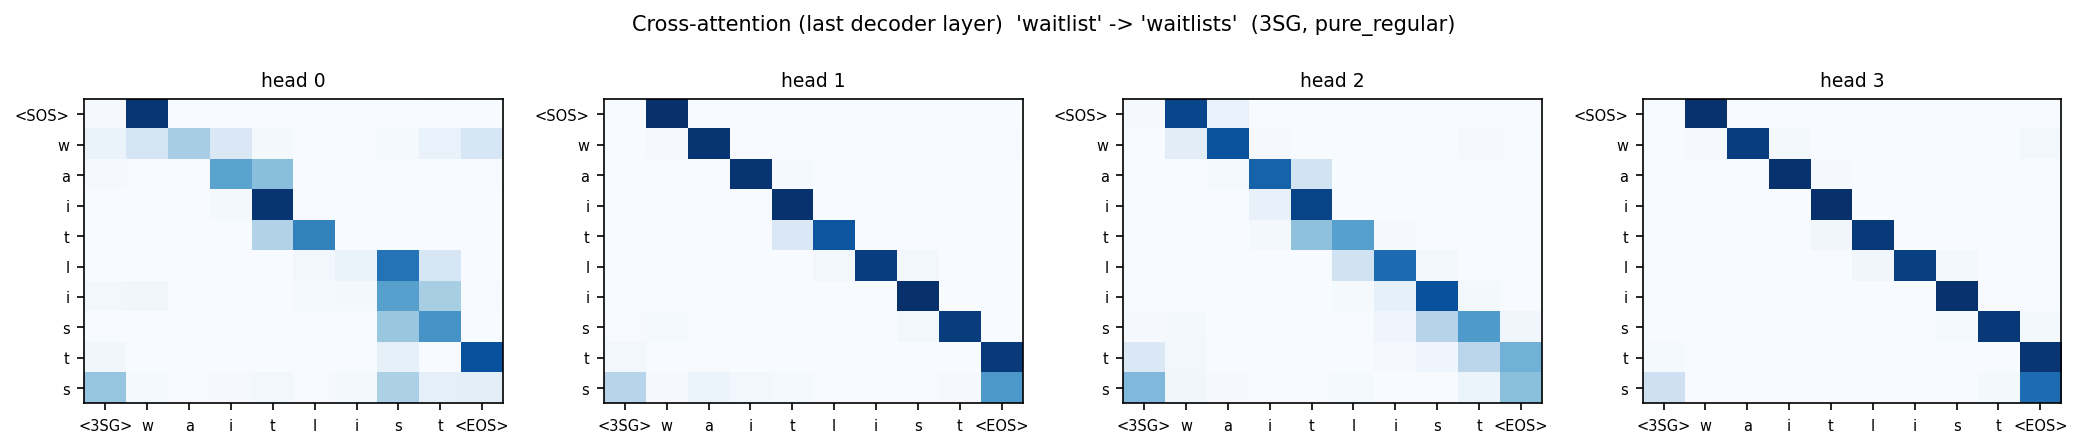
\includegraphics[width=0.48\textwidth]{labs/ch02/answers/exp4_heads/cross_attn_00_3SG_pure_regular.png}
\hfill
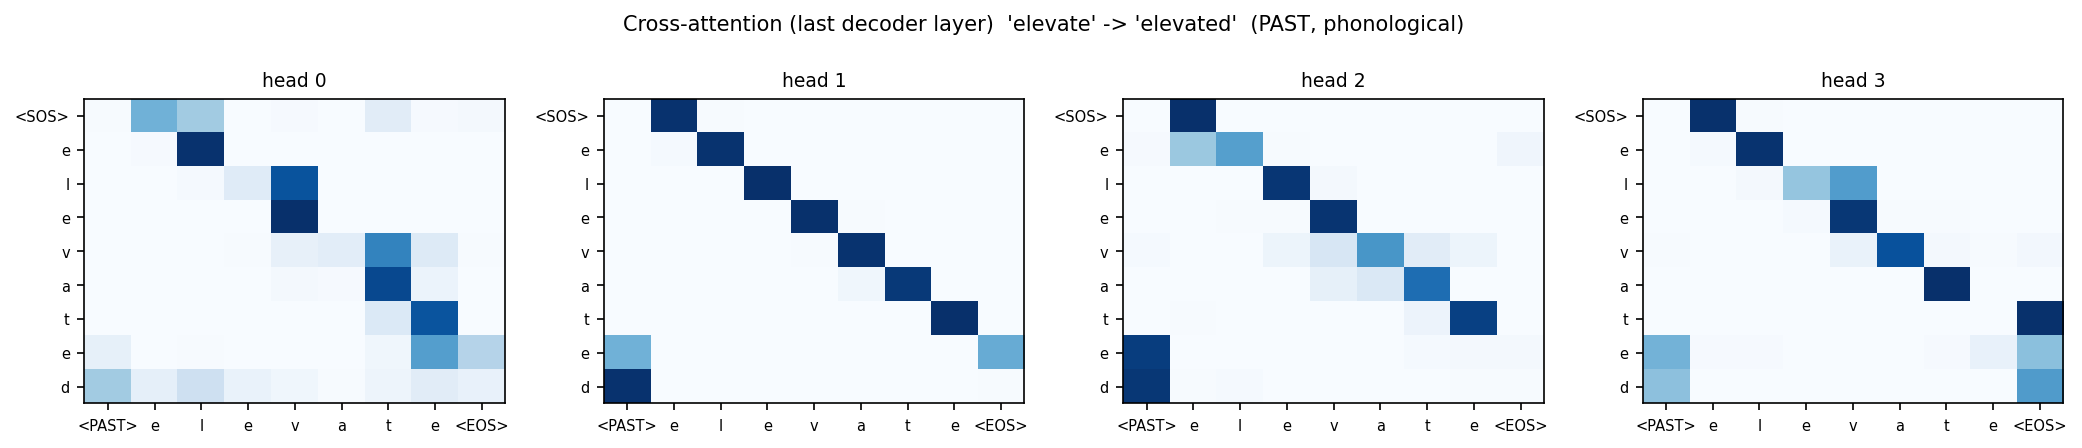
\includegraphics[width=0.48\textwidth]{labs/ch02/answers/exp4_heads/cross_attn_02_PAST_phonological.png}
\caption{Cross-attention heatmaps. Left: 3SG regular form---diagonal copy pattern visible. Right: PAST phonological form---heads attend to lemma suffix.}
\label{fig:app-lab2-heads}
\end{figure}

\textbf{Diagnosis:} Overall accuracy is robust to head count (97.0--97.1\%). The main difference is irregular accuracy: $h=1$ gets 29.8\% while $h=4$ and $h=8$ both reach 42.0\%. Multiple heads allow parallel specialization---one for copying, one for tag reading---which matters most for the hardest cases.

\textbf{Core insight:} The head visualization reveals something more important than the accuracy numbers: \emph{attention heads develop interpretable functional roles without being explicitly trained to do so}. One head learns to copy, another learns to read the tag token, another attends to suffixes. This emergent specialization is a key property of multi-head attention---it does not merely add capacity (which would help uniformly), it enables \emph{parallel decomposition of the task into sub-operations}. The accuracy data confirms this: $h=1$ suffers specifically on irregulars (which require both copying AND tag-conditioned lookup simultaneously), while regulars (which only need copying) are fine even with one head. This is why Ch3's GQA discussion matters: reducing KV heads for efficiency works because not every head needs independent keys/values---some heads can share retrieval patterns while maintaining distinct value transformations.

%----------------------------------------------------------------------
\section{Stretch Probes}

Three quick probes reusing the vanilla checkpoint:

\begin{itemize}
\item \textbf{$\sqrt{d_k}$ scaling:} Softmax entropy remains healthy as $d_k$ grows when scaling is applied; without it, entropy collapses (near-argmax behavior).
\item \textbf{Wug test:} The model generalizes productively to pseudo-words it has never seen, achieving 95.5\% accuracy---confirming it learned morphological rules, not just a lookup table.
\item \textbf{Length generalization:} Sinusoidal PE allows the model to handle longer inputs than seen in training, though accuracy degrades gracefully with length.
\end{itemize}

\begin{figure}[h]
\centering
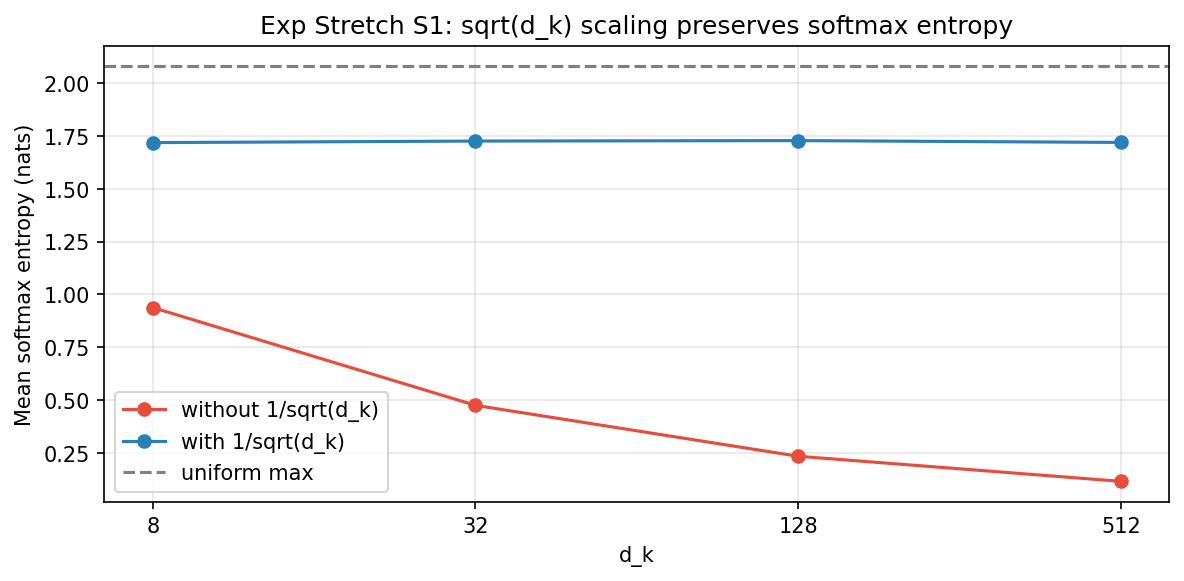
\includegraphics[width=0.6\textwidth]{labs/ch02/answers/exp_stretch/dk_softmax_entropy.png}
\caption{Softmax entropy as $d_k$ varies. Scaling preserves a healthy entropy distribution.}
\label{fig:app-lab2-dk}
\end{figure}

%----------------------------------------------------------------------
\section{Lab 2 Synthesis: Why ``Attention Is Not All You Need''}

The title of this lab is a deliberate play on the original Transformer paper's title. The experiments prove the claim:

\begin{center}
\begin{tabular}{lll}
\toprule
\textbf{Remove\ldots} & \textbf{What Breaks} & \textbf{Why} \\
\midrule
Causal mask & Train/test gap & Future leakage \\
Residual connection & Representation collapse & Averaging destroys diversity \\
FFN & Irregular/nonlinear capacity & Only linear combinations remain \\
Encoder PE & Input position awareness & Permutation-equivariant attention \\
Multi-head ($h=1$) & Irregular accuracy & Cannot parallelize sub-tasks \\
$\sqrt{d_k}$ scaling & Gradient signal & Softmax saturation \\
\bottomrule
\end{tabular}
\end{center}

\textbf{The unifying principle:} A Transformer block is not one powerful mechanism---it is a \emph{committee} of specialized mechanisms, each addressing a specific failure mode. Self-attention alone (without residual, without FFN, without proper masking and scaling) cannot learn useful representations. The supporting infrastructure is not ``boilerplate''---it is load-bearing structure.

\textbf{Connection across labs:}
\begin{itemize}
\item Lab~1 showed that recurrence without gates fails (gradient pathology, distance degradation). The solution was additive highways (cell state).
\item Lab~2 shows that attention without supporting structure fails (rank collapse, saturation, leakage). The solution is the full Transformer block: residual + FFN + mask + scaling + PE.
\item Lab~3 will show that decoder-only GPT without proper objective alignment, residual stream, and positional encoding fails. The same principle at model-architecture scale.
\end{itemize}

The recurring theme: \emph{the simplest version of each idea does not work}. What makes it work is careful engineering around the core mechanism's failure modes.
